\documentclass[12pt,a4paper,leqno]{report}

\usepackage[T1]{fontenc}
\usepackage[english]{babel}
\usepackage{amsthm}
\usepackage{amsfonts}
\usepackage{amsmath}
\usepackage{amssymb}
\usepackage{tikz}
\usepackage{listings}

\newcommand{\R}{\mathbb{R}}
\newcommand{\C}{\mathbb{C}}
\newcommand{\Q}{\mathbb{Q}}
\newcommand{\N}{\mathbb{N}}
\newcommand{\No}{\mathbb{N}_0}
\newcommand{\Z}{\mathbb{Z}}
\newcommand{\diam}{\operatorname{diam}}

\theoremstyle{plain}
\newtheorem{equa}[equation]{Equation}
\newtheorem{lem}[equation]{Lemma}
\newtheorem{prop}[equation]{Proposition}
\newtheorem{cor}[equation]{Corollary}

\theoremstyle{definition}
\newtheorem{defi}[equation]{definition}
\newtheorem{conj}[equation]{Conjecture}
\newtheorem{example}[equation]{Example}

\theoremstyle{remark}
\newtheorem{note}[equation]{Note}

\pagestyle{plain}
\makeatletter
\renewcommand{\@seccntformat}[1]{}
\makeatother
\setcounter{page}{1}
\addtolength{\hoffset}{-1.15cm}
\addtolength{\textwidth}{2.3cm}
\addtolength{\voffset}{0.45cm}
\addtolength{\textheight}{-0.9cm}

\graphicspath{ {../figures/} }

\title{Data Analytics 2 - Market Basket Analysis}
\author{Tuomo Kareoja}
\date{}

\begin{document}

\maketitle

\begin{table}[h!]
  \begin{center}
    \begin{tabular}{l|c|r}
      \textbf{Version Number} & \textbf{Changes} & \textbf{Date} \\
      \hline
      0.9 & Basic structure, text and plots & 16.09.2019\\
    \end{tabular}
  \end{center}
\end{table}

\newpage

\section{Main Takeaways}

In most product categories Blackwell and Electronidex fit together nicely by offering products in different categories or
product in different price ranges.

With PC:s, Displays and Tablets there is considerable overlap. This is worrying as these 3
categories create 45 \% percent of Blackwells' profits.

Electronidex has a huge portfolio of over 4000 products and as there are only slightly over 10000
transactions with more than 1 unique product, it is hard to find reliable connections for
buying certain products together.

If we add the product brand to the analysis, the results are still weak. The one interesting
thing in this level is the way that apple products are often bought together with other
apple products. Apple is also the most popular brand in transactions, being over 2 times
more common than the next one which OWC (who make Apple accessories).

If we perform the market basket analysis at level of product categories, we find interesting
connections between buying smartwatches, cameras and products of category other (these include
a number of different products e.g. lamps with usb ports for charging other devices, connected
thermostats etc.) and buying products of categories

\section{Blackwell Product Line Comparison to Electronidex Product Line}

Where we make profits

\bigskip
{
    \centering
    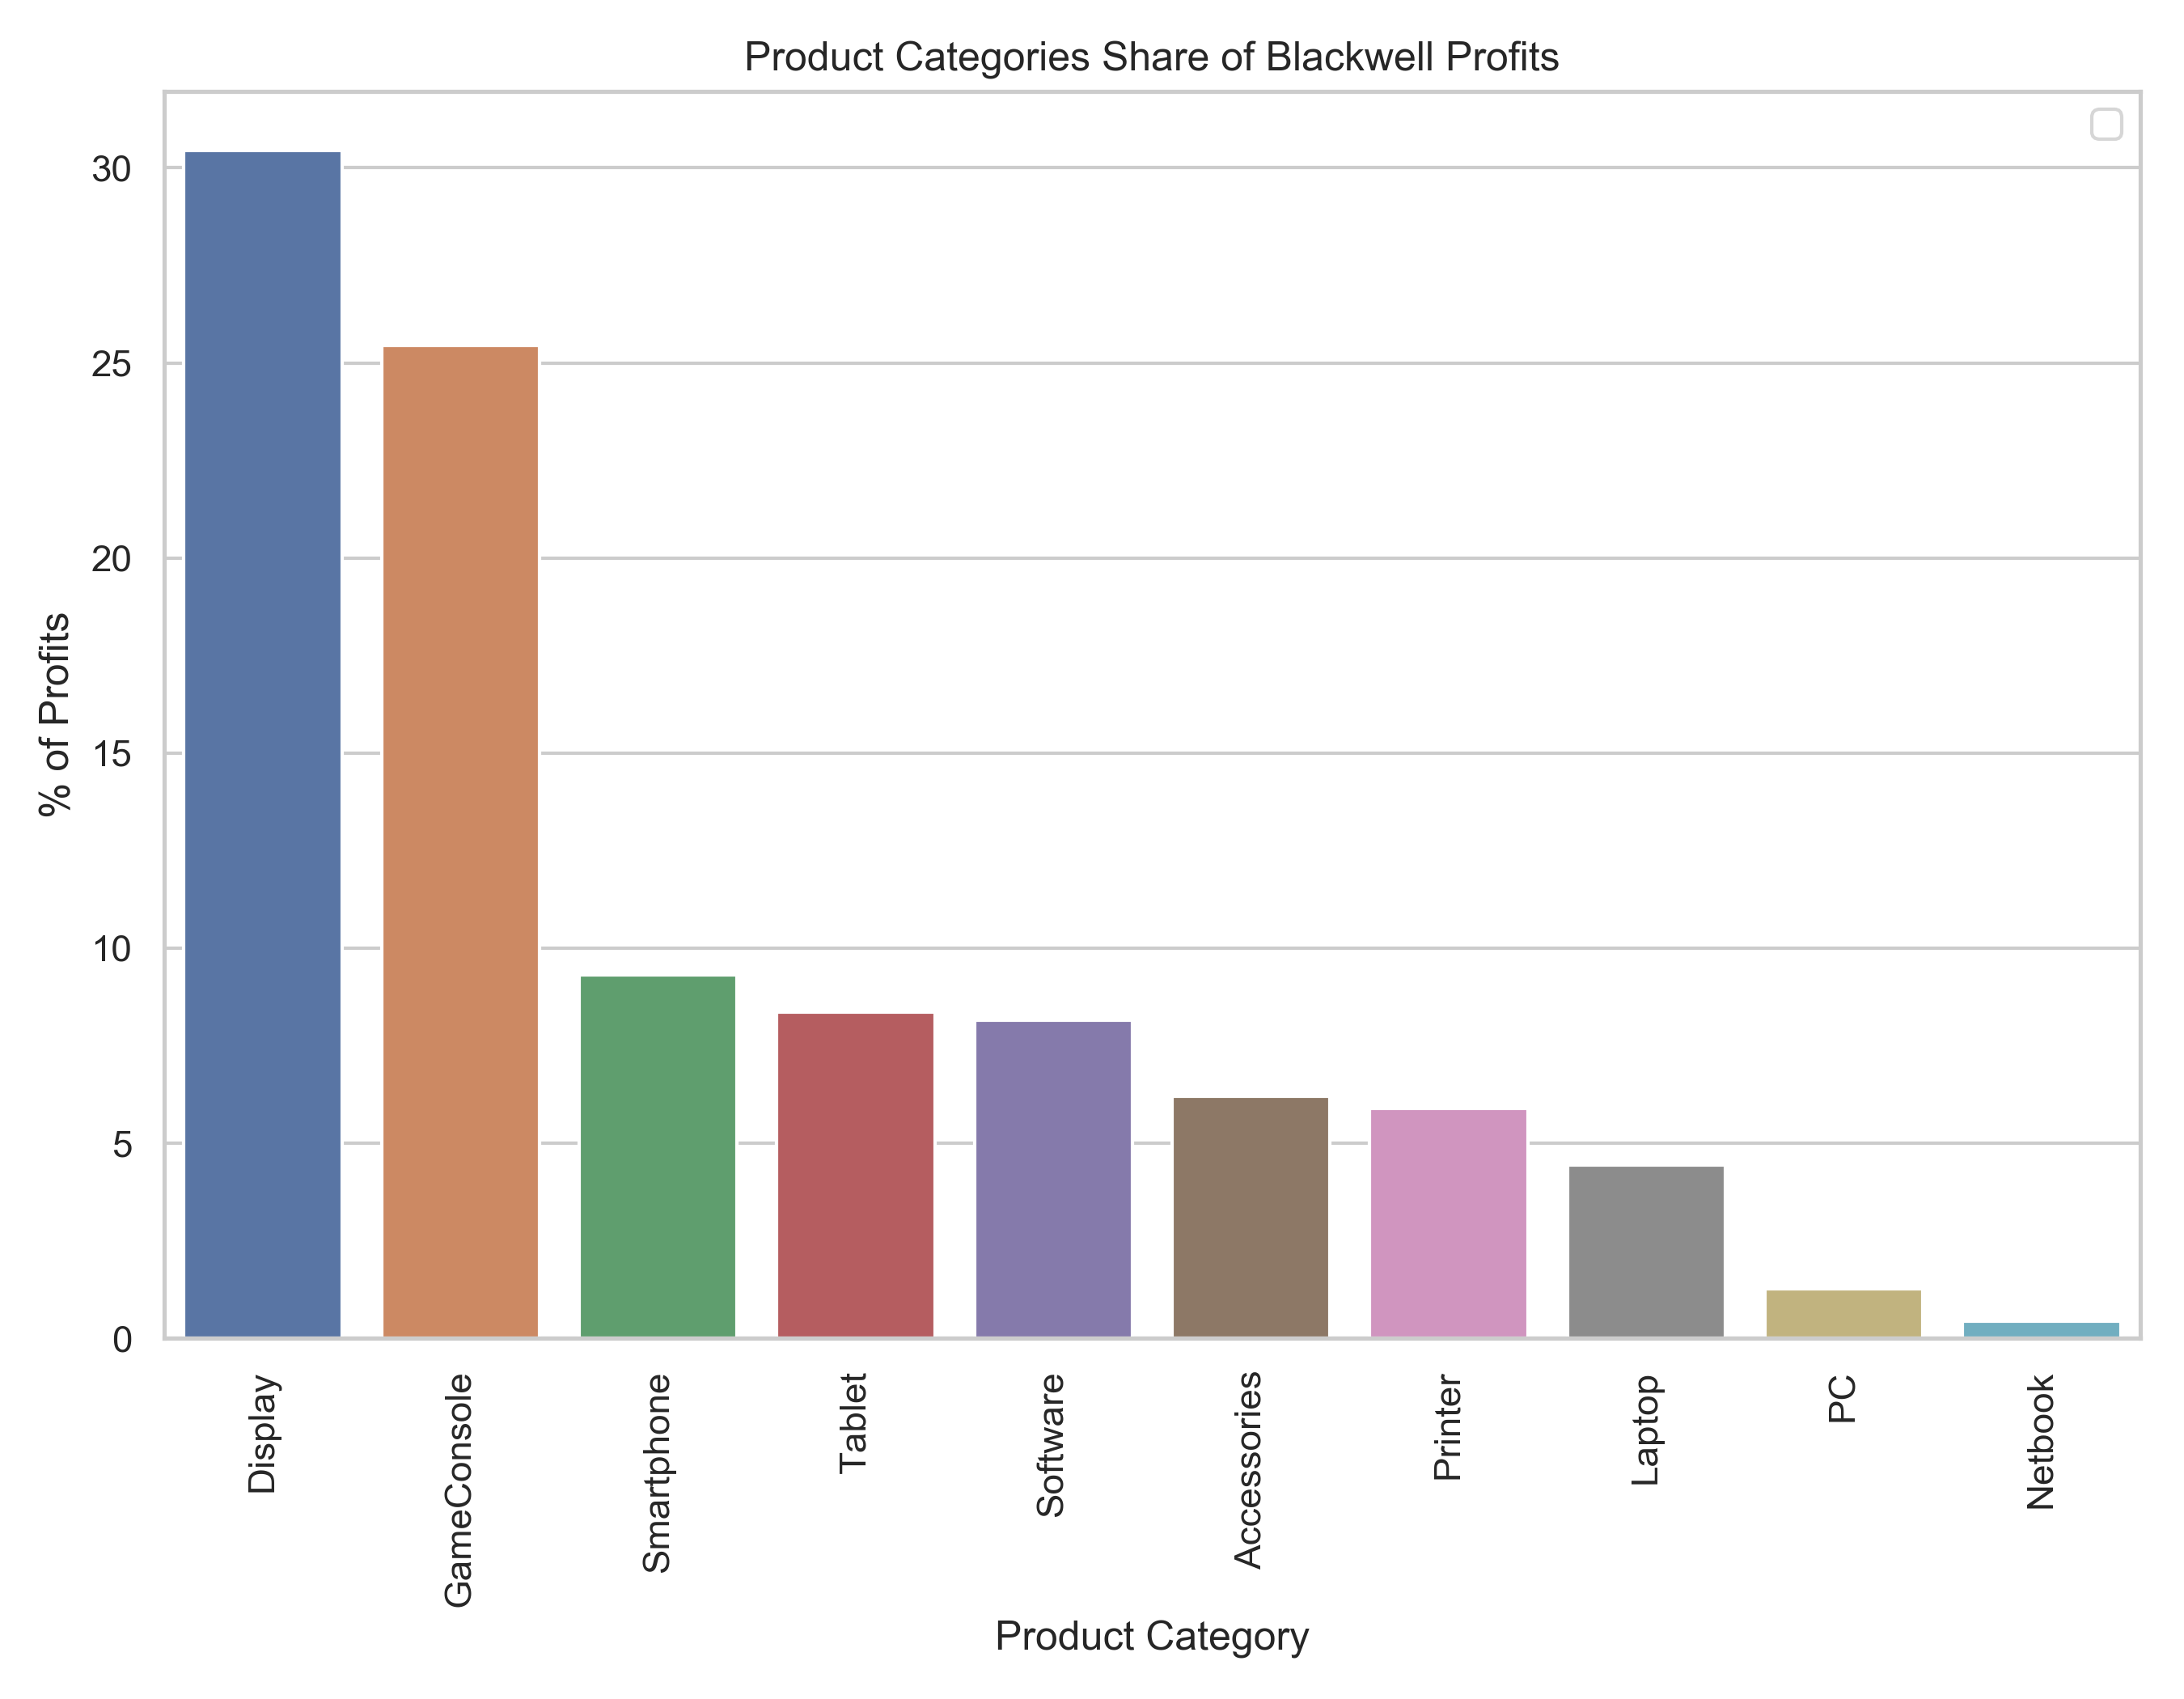
\includegraphics[width=\textwidth,height=\textheight,keepaspectratio]{blackwell_profits_share_by_product_category.png}
    \par
}
\bigskip

What are the individual profits per product?

\bigskip
{
    \centering
    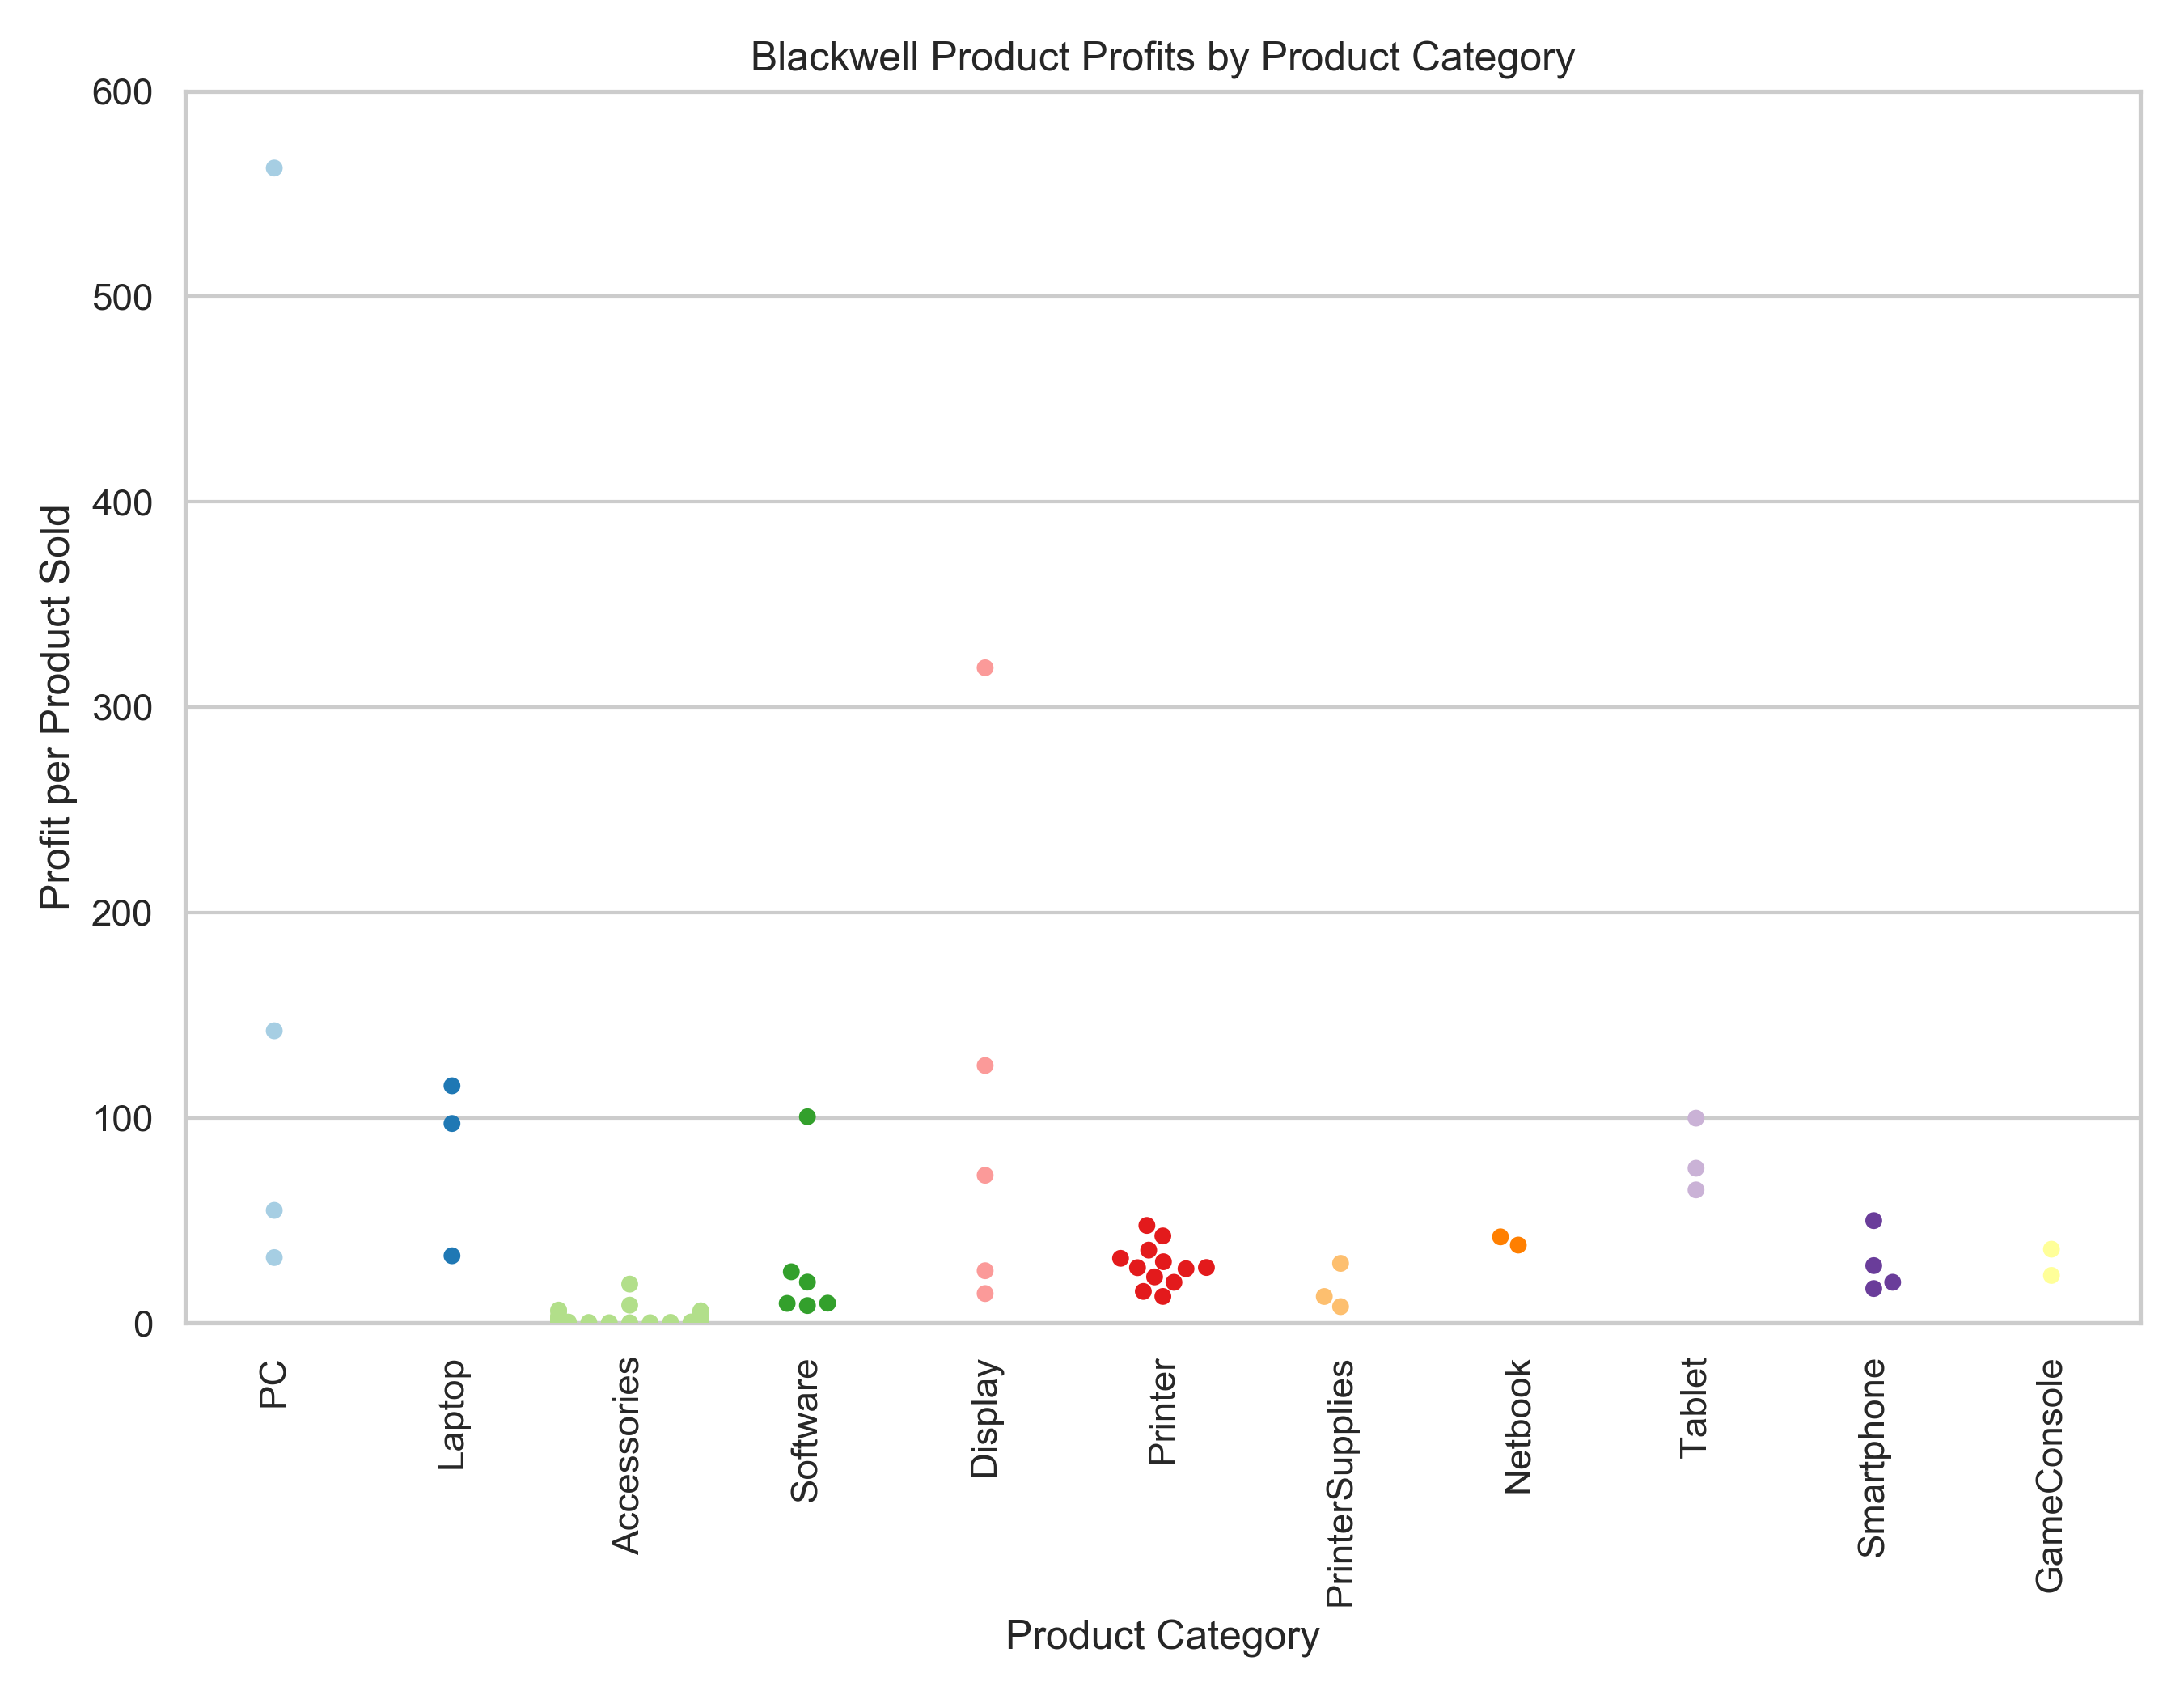
\includegraphics[width=\textwidth,height=\textheight,keepaspectratio]{blackwell_product_profitability_distribution_by_category.png}
    \par
}
\bigskip

How our product line fits in with the product line of Electronidex?

\bigskip
{
    \centering
    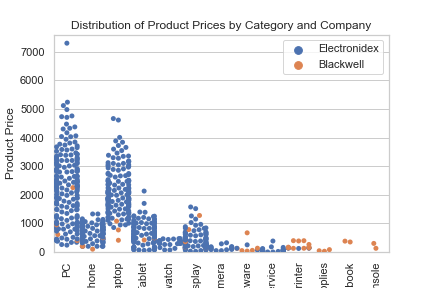
\includegraphics[width=\textwidth,height=\textheight,keepaspectratio]{product_prices_distribution_by_category_and_company.png}
    \par
}
\bigskip

Blackwell and Electronidex sales by product category

\bigskip
{
    \centering
    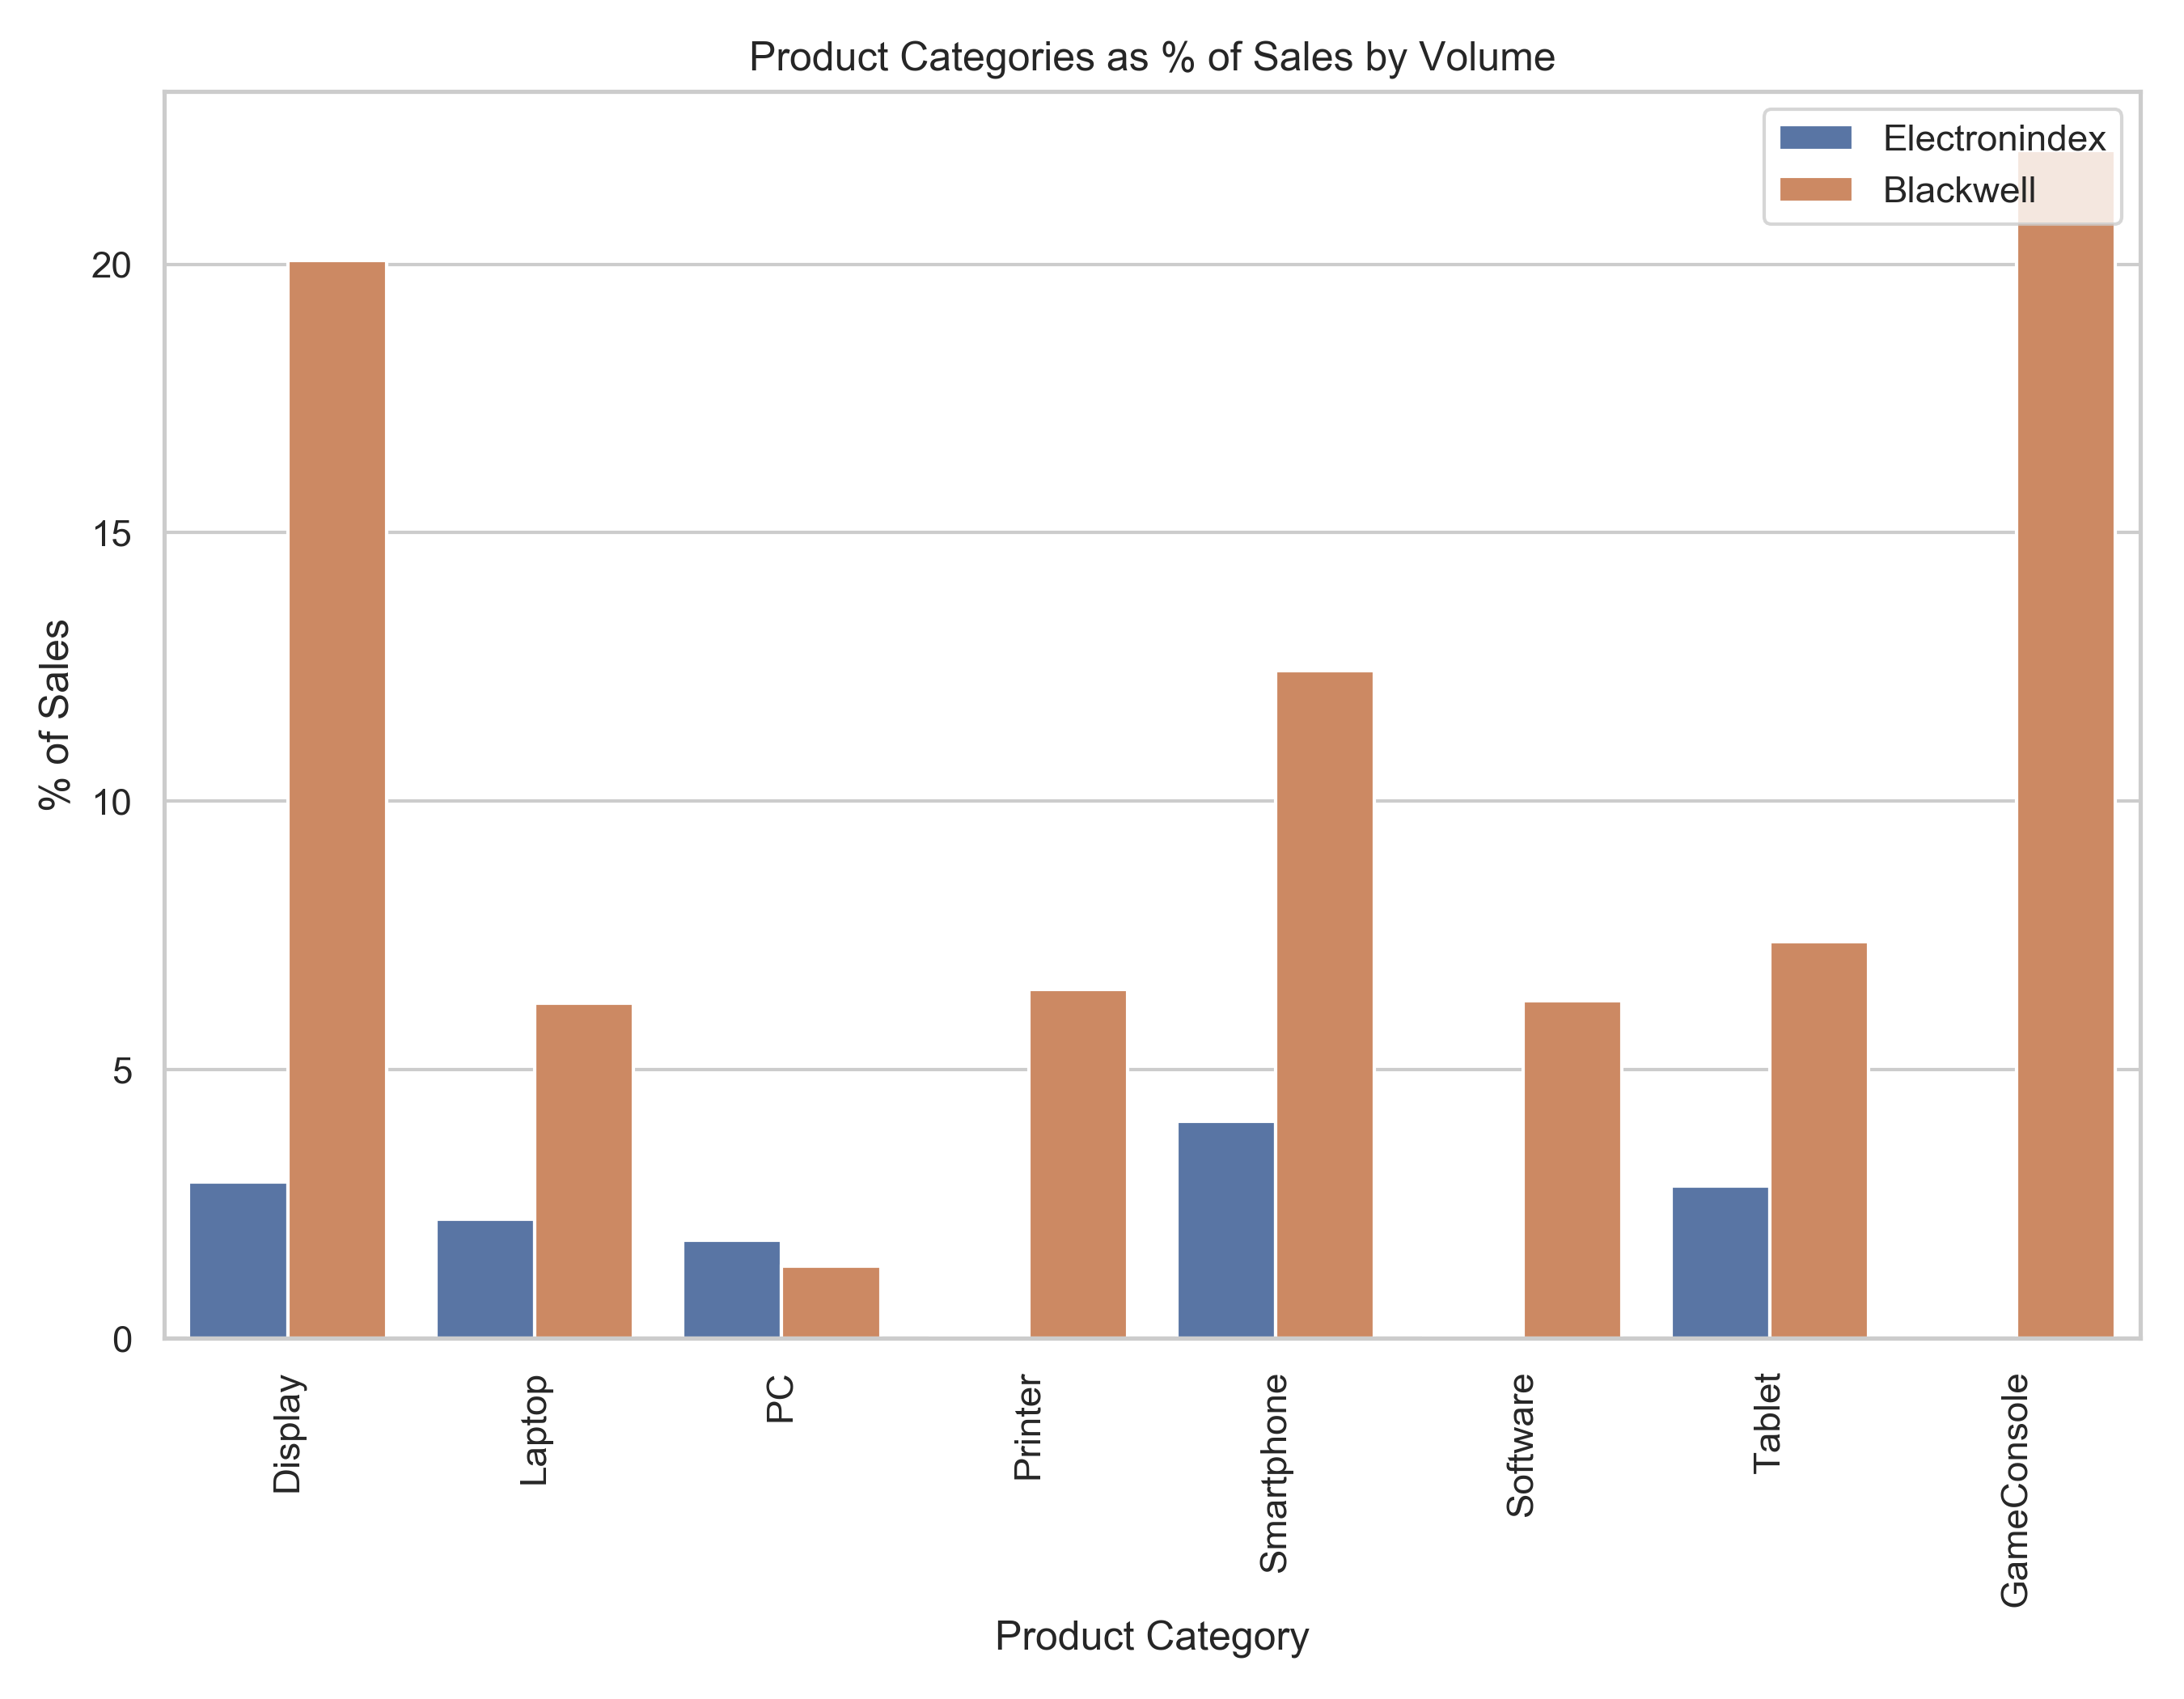
\includegraphics[width=\textwidth,height=\textheight,keepaspectratio]{sales_distribution_of_product_categories_by_volume_no_accessories.png}
    \par
}
\bigskip

\bigskip
{
    \centering
    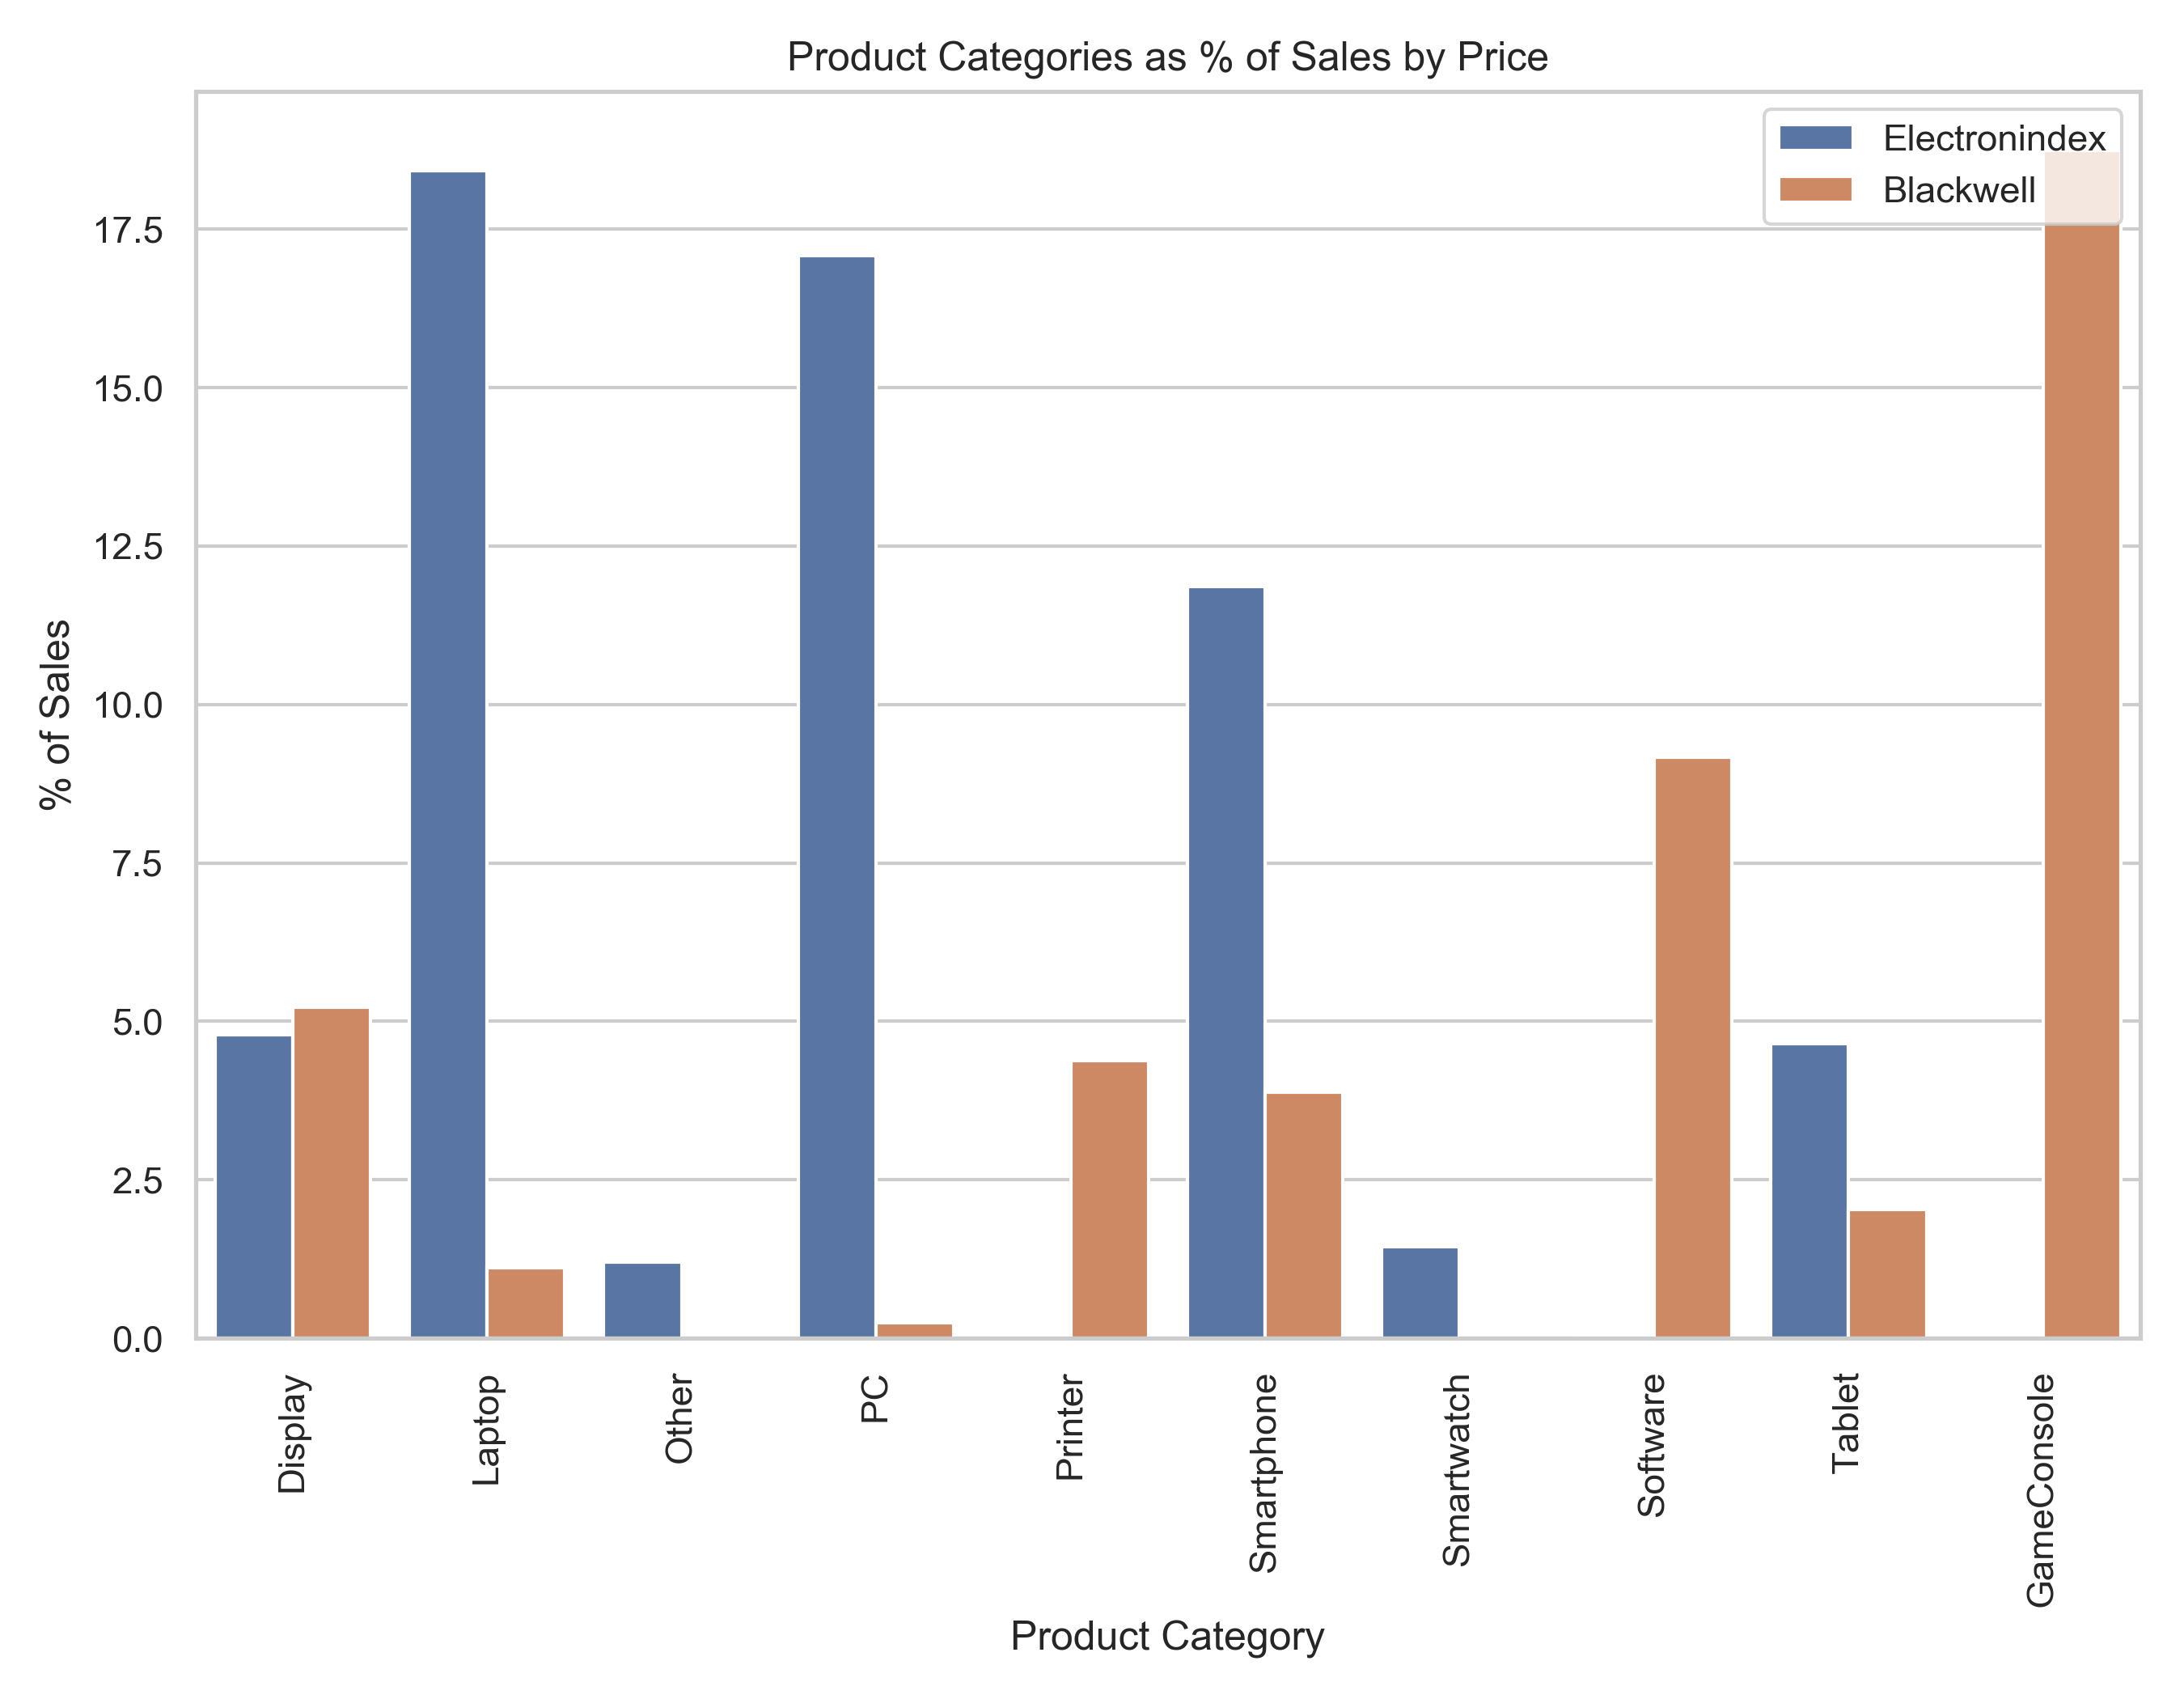
\includegraphics[width=\textwidth,height=\textheight,keepaspectratio]{sales_distribution_of_product_categories_by_price_no_accessories.png}
    \par
}
\bigskip

\section{Market Basket Analysis of Electronidex Transactions}

\subsection{Product Level}

\subsection{Brand Level}

\subsection{Product Category Level}

\end{document}
